\documentclass[11pt]{article}

\usepackage[a4paper,margin=2.4cm]{geometry}
\usepackage{amsmath,amssymb}
\usepackage{graphicx}
\usepackage{booktabs}
\usepackage{tikz}
\usetikzlibrary{arrows.meta,positioning,fit,backgrounds}
\usepackage{xcolor}
\usepackage{enumitem}
\usepackage{hyperref}
\hypersetup{colorlinks=true,linkcolor=blue!50!black,citecolor=blue!50!black,urlcolor=blue!50!black}
\usepackage[numbers,sort&compress]{natbib}
\usepackage{caption}
\usepackage{float}

\newcommand{\code}[1]{\texttt{#1}}

\title{Ego-Relative Shoulder Centerline Waypoint Generation:\\
Algorithms, Mathematical Formulation, and Implementation Report}
\author{Autoware + CARLA Shoulder Detection Project \\ \small Generated from the implementation session of 2026-07-30}
\date{2026-07-30}

\begin{document}
\maketitle
\tableofcontents

\section{Problem Statement and Scope}

The goal of this work is to generate \emph{ego-relative shoulder centerline waypoints} for an
Autoware-controlled vehicle operating in a CARLA simulation. A pre-existing package,
\code{shoulder\_detection\_ros}, runs a DINOv2-based 3-class semantic segmentation model
(\emph{travel\_lane} / \emph{shoulder} / \emph{non\_driveable}) on the front camera feed. The task
addressed in this session was to \emph{3D-ground} that 2D semantic mask, extract a smooth
centerline through the shoulder region, and publish it as a sequence of waypoints -- both as a
local, ego-relative window for a downstream planner/controller, and as a persistent, world-frame
accumulated trail for visualization and mapping.

The work is implemented as a new C++ ROS~2 package, \code{shoulder\_centerline}, chosen over Python
for execution speed and because it needed to run alongside an already GPU-contended perception
stack without adding further load.

\subsection{Available Sensor Configuration}

Both sensors used are statically transformed to \code{base\_link} (the vehicle's rear-axle,
ground-level frame) via the \code{carla\_sensor\_kit} URDF, so no online extrinsic calibration is
required -- all geometry is obtained via live \code{tf2} lookups.

\begin{itemize}[leftmargin=1.4em]
  \item \textbf{Camera} (\code{CAM\_FRONT}): static extrinsic $x{=}2.225\,\mathrm{m}$,
  $z{=}1.600\,\mathrm{m}$, zero roll/pitch/yaw relative to \code{base\_link}; live
  \code{sensor\_msgs/CameraInfo} with an ideal (distortion-free) pinhole intrinsic matrix $K$.
  \item \textbf{LiDAR} (\code{velodyne\_top}, 64-channel, 100\,m range, ray-cast model): static
  extrinsic $x{=}1.035\,\mathrm{m}$, $z{=}1.840\,\mathrm{m}$.
  \item The camera-to-optical-frame rotation follows the REP-103/ROS convention
  (roll,pitch,yaw)$=(-\pi/2,0,-\pi/2)$ from \code{camera\_link} to \code{camera\_optical\_link},
  confirmed directly from the shared \code{monocular\_camera.xacro} macro used by the sensor kit.
\end{itemize}

\section{System Architecture}

\begin{figure}[H]
\centering
\resizebox{\linewidth}{!}{%
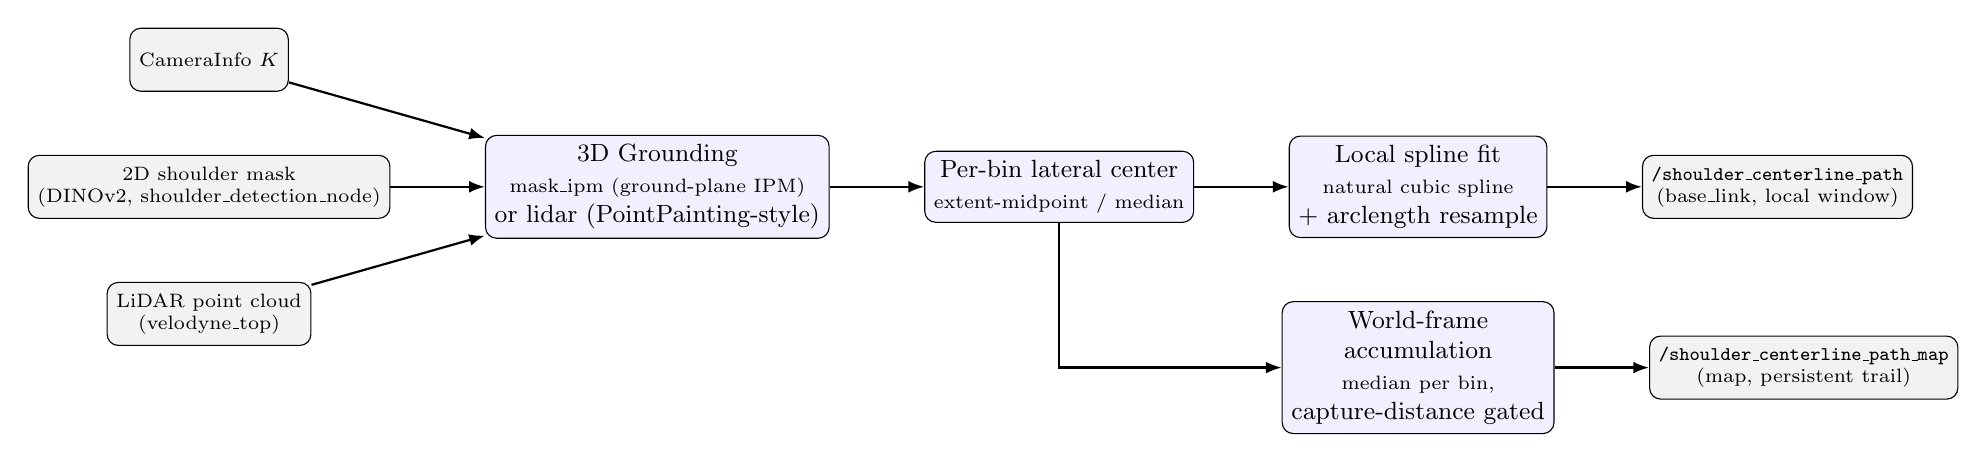
\begin{tikzpicture}[
  node distance=8mm and 12mm,
  block/.style={draw, rounded corners, fill=blue!6, align=center, minimum height=9mm, font=\small},
  io/.style={draw, rounded corners, fill=gray!10, align=center, minimum height=8mm, font=\scriptsize},
  arr/.style={-{Latex[length=2mm]}, thick}
]
\node[io] (mask) {2D shoulder mask\\\scriptsize(DINOv2, shoulder\_detection\_node)};
\node[io, below=of mask] (lidar) {LiDAR point cloud\\\scriptsize(velodyne\_top)};
\node[io, above=of mask] (caminfo) {CameraInfo $K$};

\node[block, right=of mask] (ground) {3D Grounding\\\scriptsize mask\_ipm (ground-plane IPM)\\ or lidar (PointPainting-style)};
\node[block, right=of ground] (center) {Per-bin lateral center\\\scriptsize extent-midpoint / median};
\node[block, right=of center] (spline) {Local spline fit\\\scriptsize natural cubic spline\\+ arclength resample};
\node[block, below=of spline] (world) {World-frame\\accumulation\\\scriptsize median per bin,\\capture-distance gated};

\node[io, right=of spline] (local) {\code{/shoulder\_centerline\_path}\\\scriptsize(base\_link, local window)};
\node[io, right=of world] (global) {\code{/shoulder\_centerline\_path\_map}\\\scriptsize(map, persistent trail)};

\draw[arr] (mask) -- (ground);
\draw[arr] (lidar) -- (ground);
\draw[arr] (caminfo) -- (ground);
\draw[arr] (ground) -- (center);
\draw[arr] (center) -- (spline);
\draw[arr] (spline) -- (local);
\draw[arr] (center.south) |- (world.west);
\draw[arr] (world) -- (global);
\end{tikzpicture}%
}
\caption{Per-frame processing pipeline. Both outputs share the same 3D-grounding and per-bin
lateral-centering stages; they diverge only in how the resulting samples are turned into
published waypoints (Sections~\ref{sec:local} and \ref{sec:world}).}
\end{figure}

\section{3D Grounding of the 2D Semantic Mask}
\label{sec:grounding}

Two independent methods were implemented and compared, selectable at launch time via the
\code{bin\_source} parameter.

\subsection{Method A: LiDAR Semantic Painting (PointPainting-style)}
\label{sec:pointpainting}

The first method follows the \emph{sequential fusion} idea of PointPainting
\citep{vora2020pointpainting}, also used inside Autoware itself as the
\code{pointpainting\_fusion} package of \code{autoware\_image\_projection\_based\_fusion}: each
LiDAR point is projected into the camera image and \emph{painted} with the semantic class found
at its projected pixel.

\paragraph{Projection.} For a LiDAR point $\mathbf{p}_{L}$ in the LiDAR frame, the live
\code{tf2}-derived rigid transform $T_{C \leftarrow L} = (R_{CL}, \mathbf{t}_{CL})$ into the camera
optical frame gives
\begin{equation}
\mathbf{p}_C = R_{CL}\,\mathbf{p}_L + \mathbf{t}_{CL} = (X_C, Y_C, Z_C)^\top .
\end{equation}
The pixel coordinates follow the standard pinhole model,
\begin{equation}
u = f_x \frac{X_C}{Z_C} + c_x, \qquad
v = f_y \frac{Y_C}{Z_C} + c_y,
\label{eq:pinhole}
\end{equation}
valid only when $Z_C > \epsilon$ ($\epsilon{=}0.1\,\mathrm{m}$, rejecting points behind or
extremely close to the camera plane) and $(u,v)$ within the image bounds. The point is
\emph{painted} shoulder if the mask value at $(u,v)$ equals the shoulder class index.

\paragraph{Ground banding.} Painted points are then transformed into \code{base\_link} via
$T_{B \leftarrow L}$ and retained only if their height $z_B \in [z_{\min}, z_{\max}] =
[-0.3, 0.5]\,\mathrm{m}$ and forward distance $x_B \in [x_{\min}, x_{\max}] = [3, 40]\,\mathrm{m}$,
rejecting mask bleed onto off-ground clutter (guardrails, vegetation) and points outside the
region of interest.

\paragraph{Observed limitation.} On a genuinely narrow shoulder (e.g.\ a mountain-pass section
with $\sim$1--1.5\,m of paved shoulder before a guardrail), only a handful of the LiDAR's discrete
scan rays land inside the shoulder region per frame ($\sim$30--40 painted points spread across the
full 3--40\,m range in the deployed configuration). This sparsity, not the choice of per-bin
aggregator, was empirically identified as the dominant source of centerline noise on narrow
sections (Section~\ref{sec:estimator}).

\subsection{Method B: Monocular Mask-Boundary Inverse Perspective Mapping}
\label{sec:ipm}

To avoid the LiDAR sparsity problem, a second method works directly in the dense 2D mask and uses
classical \emph{inverse perspective mapping} (IPM) \citep{ipm2021,ipm2026} -- the same principle
underlying most monocular lane-centering ADAS systems -- to back-project a single boundary-derived
pixel per image row onto the ground plane, rather than relying on sparse LiDAR returns at all.

\paragraph{Step 1 -- largest contiguous mask run per row.} For each sampled image row
(every \code{mask\_row\_step} rows), the largest contiguous run of shoulder-classified columns is
found by a single left-to-right scan tracking run start/length (a one-dimensional connected-component
scan). Using the \emph{largest} run, rather than the global min/max classified column, makes this
robust to disjoint false-positive detections elsewhere in the same row -- a naive min/max would
wrongly span across two unrelated regions. Runs shorter than \code{min\_mask\_run\_px} (default 3)
are rejected as pixel-level mask noise. The run's midpoint column is taken as the row's
shoulder-center pixel:
\begin{equation}
u_c = u_{\text{start}} + \tfrac{1}{2}(\ell - 1), \qquad \ell = \text{run length}.
\end{equation}

\paragraph{Step 2 -- ground-plane back-projection.} Given the live camera pose
$T_{B \leftarrow C} = (R_{BC}, \mathbf{t}_{BC})$ in \code{base\_link}, the pixel $(u_c, v)$ defines
an (unnormalized) ray direction in the camera optical frame,
\begin{equation}
\mathbf{d}_C = \left( \frac{u_c - c_x}{f_x},\ \frac{v - c_y}{f_y},\ 1 \right)^\top,
\end{equation}
rotated into \code{base\_link} as $\mathbf{d}_B = R_{BC}\,\mathbf{d}_C$. Assuming a locally flat
ground plane $z_B = 0$ (consistent with this project's documented flat CARLA test routes), the
ray-plane intersection parameter is
\begin{equation}
t^\ast = \frac{-\,t_{BC,z}}{d_{B,z}}, \qquad \text{valid only if } d_{B,z} < -\eta \text{ and } t^\ast > 0,
\end{equation}
($\eta{=}10^{-6}$, rejecting rays parallel to or above the horizon), giving the grounded point
\begin{equation}
\mathbf{p}_B = \mathbf{t}_{BC} + t^\ast \mathbf{d}_B = (x_B, y_B, 0)^\top.
\end{equation}

This method is dense (one candidate sample per sampled image row, regardless of how narrow the
real shoulder is) at the cost of the flat-ground assumption, and became the default
(\code{bin\_source=mask\_ipm}).

\section{Lateral Centerline Estimation per Forward-Distance Bin}
\label{sec:estimator}

Grounded samples (from either Section~\ref{sec:pointpainting} or \ref{sec:ipm}) are binned by
forward distance into fixed-width bins of size \code{bin\_size} ($1.0\,\mathrm{m}$) spanning
$[x_{\min}, x_{\max}]$. A bin is only used once it holds at least \code{min\_points\_per\_bin}
samples.

\subsection{Baseline: Density-Weighted Median}
A first implementation took the ordinary median of each bin's lateral ($y$) samples,
\begin{equation}
\hat{y} = \operatorname{median}\{y_1,\dots,y_n\}.
\end{equation}
This is a \emph{density-weighted centroid}: whichever edge of the shoulder happens to receive more
LiDAR hits or mask-boundary samples (a function of scan pattern/incidence angle, not of the lane's
true geometric width) pulls the estimate toward it. This was confirmed visually: the centerline
consistently sat off-center toward one edge of the shoulder strip.

\subsection{Robust Extent-Midpoint Estimator}
Classical lane-detection literature instead constructs the lane centerline as the midpoint between
the detected left and right lane boundaries -- the sliding-window/histogram lane-finding technique
common in monocular lane detection, and the general principle that ``the lane-center line is
calculated as the average between the left and right lane boundary''. Adapting this here: sort the
bin's samples, trim the extreme \code{edge\_trim\_fraction} (default $0.1$) from each end to reject
outliers, and take the midpoint of what remains,
\begin{equation}
\hat{y} = \tfrac{1}{2}\big( y_{(\lceil fn \rceil)} + y_{(n - \lceil fn \rceil)} \big),
\label{eq:extentmid}
\end{equation}
where $y_{(1)} \le \dots \le y_{(n)}$ are the sorted samples and $f$ is the trim fraction. This
directly targets the geometric extent of the classified region rather than its sample density, and
became the default (\code{centerline\_estimator=extent\_midpoint}).

\section{Local Ego-Relative Path Construction}
\label{sec:local}

\subsection{Natural Cubic Spline Fit}
The $n$ valid bin centers $(x_i, \hat{y}_i)_{i=0}^{n-1}$ (bin centers are uniformly spaced by
construction) are fit with a \emph{natural cubic spline} using a uniform-knot parametrization
$t = 0,1,\dots,n-1$ -- the textbook tridiagonal (Thomas-algorithm) formulation
\citep{numericalrecipes}, implemented independently for $x(t)$, $y(t)$, $z(t)$.

Let $M_i = f''(t_i)$ denote the second derivatives at the knots. The natural boundary condition
sets $M_0 = M_{n-1} = 0$; the interior values solve the tridiagonal system
\begin{equation}
M_{i-1} + 4 M_i + M_{i+1} = 6\big(y_{i+1} - 2y_i + y_{i-1}\big), \qquad i = 1,\dots,n-2,
\end{equation}
solved via forward elimination / back substitution (Thomas algorithm) in $O(n)$. Within segment
$[i, i{+}1]$, with local parameter $s = t - i \in [0,1]$,
\begin{align}
f(s) &= y_i(1{-}s) + y_{i+1}s + \big[(1{-}s)^3 - (1{-}s)\big]\tfrac{M_i}{6} + \big(s^3-s\big)\tfrac{M_{i+1}}{6}, \\
f'(s) &= (y_{i+1}-y_i) + \big[{-}3(1{-}s)^2+1\big]\tfrac{M_i}{6} + \big(3s^2-1\big)\tfrac{M_{i+1}}{6}, \\
f''(s) &= M_i(1{-}s) + M_{i+1}s.
\end{align}
This uniform-knot parametrization is a documented simplification relative to a chord-length
parametrization: accurate as long as valid bins are mostly contiguous (the common case here).

\subsection{Arclength Resampling}
The fitted curve is densely sampled ($20$ sub-samples per knot interval), and the cumulative
Euclidean arclength
\begin{equation}
s_k = \sum_{j=1}^{k} \sqrt{(x_j - x_{j-1})^2 + (y_j - y_{j-1})^2}
\end{equation}
is tabulated. Waypoints are then produced at fixed arclength spacing \code{waypoint\_spacing}
($1.0\,\mathrm{m}$) by inverting this table (linear interpolation) to find the corresponding knot
parameter $t$.

\subsection{Frenet-Frame Heading and Curvature}
At each resampled waypoint, heading and signed curvature follow the standard Frenet-frame
formulas,
\begin{equation}
\psi = \operatorname{atan2}(y', x'), \qquad
\kappa = \frac{x'y'' - y'x''}{\left(x'^2+y'^2\right)^{3/2}},
\label{eq:curvature}
\end{equation}
using the spline's analytic first/second derivatives at the resampled parameter value.

\subsection{Temporal Smoothing}
An exponential moving average is applied per arclength-index across frames,
\begin{equation}
\hat{y}^{(t)}_k = \alpha\, y^{(t)}_k + (1-\alpha)\, \hat{y}^{(t-1)}_k, \qquad \alpha = \code{smoothing\_alpha},
\end{equation}
keyed by the waypoint's discrete arclength step $k$ -- a lightweight, per-index low-pass filter
appropriate for a compute budget that must not add further GPU load on an already
contention-limited machine.

This local path is deliberately \emph{not} filtered by any of the robustness mechanisms in
Section~\ref{sec:refinements}: it is re-derived from scratch every frame, so an occasional bad
frame is self-healing, and an earlier attempt to filter it caused a measurable regression (shorter,
wrongly-trimmed paths), documented in Section~\ref{sec:refinements}.

\section{World-Frame Persistent Accumulation}
\label{sec:world}

The local path above is an ego-relative window that RViz redraws from scratch every message (by
design -- a local planner/controller wants the current-frame view, not history). For
visualization and mapping, a second, persistently \emph{accumulating} path is built directly from
the raw grounded samples, independent of the local spline fit.

\subsection{Traveled-Arclength Keying}
Rather than a 2D spatial grid (which would require handling curvature/heading explicitly), world
bins are keyed by a scalar: the vehicle's own cumulative traveled distance plus the sample's
ego-relative forward offset at capture time,
\begin{equation}
\texttt{traveled\_arclength} \mathrel{+}= \lVert \mathbf{e}_t - \mathbf{e}_{t-1} \rVert_2,
\qquad
k_{\text{world}} = \left\lfloor \frac{\texttt{traveled\_arclength} + x_{\text{sample}}}{\text{bin\_size}} \right\rfloor,
\end{equation}
where $\mathbf{e}_t$ is the ego's map-frame $(x,y)$ position from $T_{M \leftarrow B}$ at frame
$t$. This key is monotonic along the route and robust to curvature without any Frenet/heading
reconstruction.

\subsection{Multi-Sweep Accumulation}
Every sample whose world key maps to a given bin is stored (as raw $(x,y,z)$ map-frame
coordinates); the published position for that bin is the per-axis median (Eq.~\ref{eq:extentmid}
for $y$) of \emph{every} sample ever collected, once the bin holds at least
\code{min\_world\_bin\_samples}. Because a fixed real-world segment stays inside the
$[x_{\min},x_{\max}]$ window for the vehicle's entire approach -- on the order of $50$--$100+$
frames -- each world bin accumulates far more independent observations than any single frame's
estimate, analogous to standard multi-sweep LiDAR/scan accumulation in mapping pipelines: averaging
many independent noisy observations is a fundamentally more robust estimator than smoothing one
frame's sparse fit.

\section{Iterative Robustness Refinements and Lessons Learned}
\label{sec:refinements}

The accumulated path went through several rounds of diagnosis and refinement over the course of
the session; the unsuccessful attempts are documented here alongside the successful one, since the
negative results meaningfully constrain the design space.

\subsection{Attempt 1: Theil--Sen Robust Regression (reverted)}
An early symptom was a short run of bins reversing sign in the local fit's slope -- with only a
handful of valid bins, a natural cubic spline has almost no averaging effect and faithfully follows
noise in the least-densely-sampled bins. The Theil--Sen estimator
\citep{theil1950,sen1968} -- the median of all pairwise slopes, tolerant of up to $\sim$29\% of
points being arbitrary outliers -- was used to fit a robust trend through each frame's valid bins,
\begin{equation}
\hat{m} = \operatorname{median}_{i<j} \left( \frac{y_j - y_i}{x_j - x_i} \right), \qquad
\hat{b} = \operatorname{median}_i \left( y_i - \hat{m} x_i \right),
\label{eq:theilsen}
\end{equation}
and bins whose residual from this line exceeded a threshold were rejected. \textbf{Outcome:}
initially applied to both the local fit and the accumulated path, this caused a regression (a
visibly shorter, wrongly-trimmed local path), because with the small bin counts typical here,
Theil--Sen's own robustness breaks down (a 2-of-5 outlier minority is already near the estimator's
statistical breakdown point). Restricting the rejection to gate only the accumulated path did not
fully resolve the user-observed issue either, and the whole mechanism was reverted at the user's
request.

\subsection{Attempt 2: Rank-Based Near/Far Margin Exclusion (reverted)}
A follow-up hypothesis was that the \emph{farthest} (then, after correction, the \emph{nearest})
currently-valid bin each frame is the least-confirmed and should be excluded from world
accumulation. This was implemented as a positional trim of the valid-bin list (by rank, not by
absolute distance). \textbf{Outcome:} frame-by-frame video analysis (Section~\ref{sec:validation})
showed the shift was not confined to a single rank-identified bin -- a whole established stretch of
the accumulated trail could be offset, which a relative, frame-dependent rank criterion cannot
address. Reverted at the user's request after two correction attempts.

\subsection{Attempt 3: Absolute Capture-Distance Gate (adopted)}
The key realization: the bias is tied to genuinely short \emph{absolute} range, not to whichever
bin currently ranks nearest or farthest. Monocular IPM (Section~\ref{sec:ipm}) uses a
near-vertical ray at short range, so small mask-boundary pixel noise maps to a disproportionately
large swing in the back-projected ground point -- a documented limitation of monocular IPM
\citep{ipm2021}. Since every world bin passes through this same short-range window at some point
during its approach, the bias is \emph{systematic}, not a one-off outlier, which explains why a
whole stretch of the trail (not just the newest tip) could appear shifted. The fix gates
individual raw samples by their own absolute capture-time forward distance, independent of bin
rank:
\begin{equation}
\text{sample accepted into world accumulation} \iff x_{\text{sample}} \ge x_{\text{trust}}
= \code{world\_min\_capture\_x} = 10.0\,\mathrm{m}.
\label{eq:capturegate}
\end{equation}
\textbf{Outcome:} confirmed effective by the quantitative validation in
Section~\ref{sec:validation} -- the long, already-settled middle of the accumulated trail shows
sub-decimeter deviation, consistent with the systematic near-range bias having been removed.

\section{Empirical Validation}
\label{sec:validation}

\subsection{Diagnostic Instrumentation}
Throughout the session, a per-frame diagnostic counter chain was used to localize failures without
guessing:
\begin{center}
\code{lidar\ total} $\to$ \code{in\_img} $\to$ \code{painted} $\to$ \code{banded} $\to$ \code{bins valid/total} $\to$ \code{waypoints}
\end{center}
This proved the fastest way to distinguish "no data reaching the pipeline" (a real bug, found once)
from "data reaching the pipeline but of low quality" (a tuning/algorithm problem, the recurring
theme of Sections~\ref{sec:estimator}--\ref{sec:refinements}). Screencasts of the running system
were also decomposed frame-by-frame with \code{ffmpeg} (\code{fps} filter, dense frame extraction)
when a static screenshot was ambiguous about whether an artifact was ego-relative (moving with the
vehicle -- implicating the local fit) or world-fixed (implicating a real road feature).

\subsection{Quantitative Deviation Analysis}
To move past visual inspection, the live accumulated path was dumped via a direct \code{rclpy}
subscriber (the \code{ros2 topic echo} CLI truncates long array fields and is unsuitable for this)
and the local perpendicular deviation of each point from a straight line through its $\pm4$
neighbors was computed,
\begin{equation}
\text{dev}_i = \frac{(\mathbf{p}_i - \mathbf{p}_{i-w}) \times (\mathbf{p}_{i+w} - \mathbf{p}_{i-w})}
{\lVert \mathbf{p}_{i+w} - \mathbf{p}_{i-w} \rVert}, \qquad w = 4.
\end{equation}
Figure~\ref{fig:deviation} shows the result on a live capture: the long, fully-matured middle
section of the trail (roughly indices 34--118) has deviation consistently under $0.1\,\mathrm{m}$,
while both the oldest end (accumulated right after node startup, before any bin had a full
approach history) and the newest end (the still-forming growing tip nearest the vehicle) show
deviations up to $0.7\,\mathrm{m}$. This confirmed the capture-distance gate
(Eq.~\ref{eq:capturegate}) was correcting the systematic bias in already-settled bins, and reframed
the remaining roughness as an inherent \emph{maturation latency} (a bin needs enough accumulated
distance/samples to converge) rather than a remaining bias -- addressable by raising
\code{min\_world\_bin\_samples} rather than further sample-level filtering.

\begin{figure}[H]
\centering
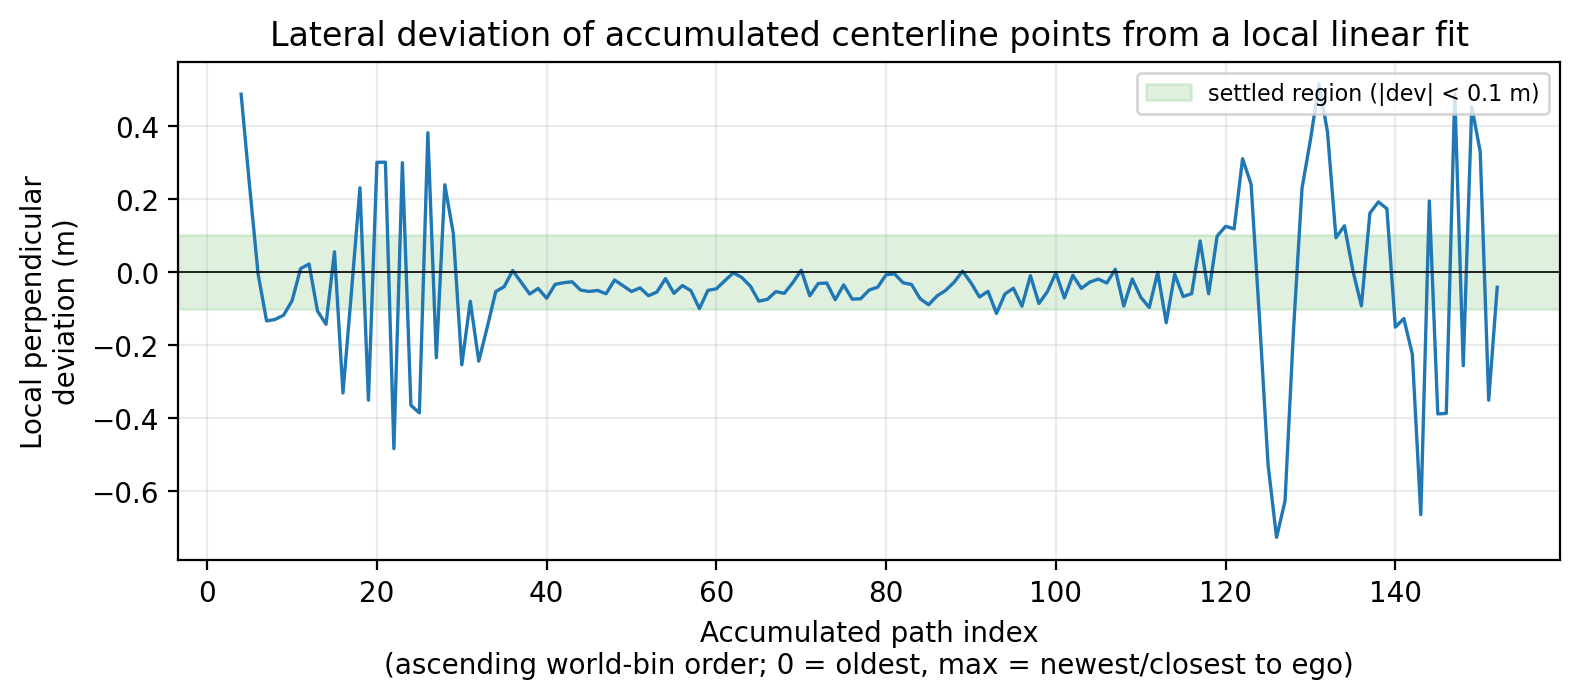
\includegraphics[width=0.95\linewidth]{figs/fig_deviation_plot.png}
\caption{Local perpendicular deviation along one live accumulated-path capture (149 points). The
settled middle section (green band, $|\text{dev}| < 0.1\,\mathrm{m}$) is markedly cleaner than
both ends, which are still within their maturation window.}
\label{fig:deviation}
\end{figure}

\subsection{Visual Results}

\begin{figure}[H]
\centering
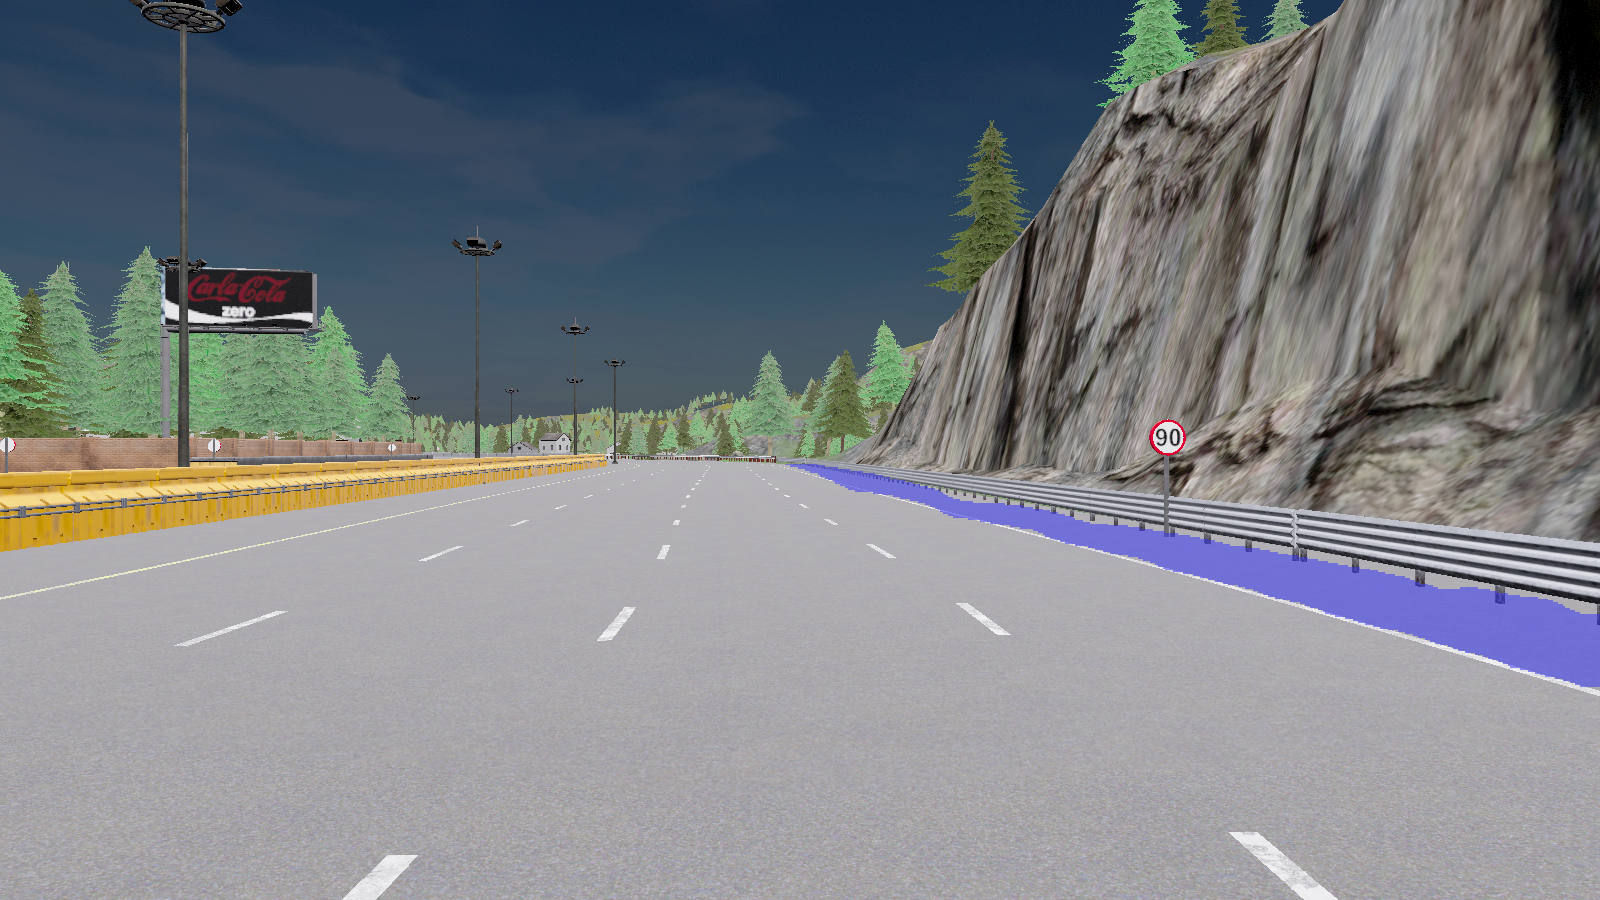
\includegraphics[width=0.75\linewidth]{figs/fig_mask_overlay.png}
\caption{Input: the 3-class semantic overlay (green = travel lane, blue = shoulder, red =
non-driveable) on a narrow mountain-pass section, showing a genuinely narrow ($\sim$1--1.5\,m)
paved shoulder before a guardrail -- the case that motivated the mask-IPM method
(Section~\ref{sec:ipm}) over LiDAR painting alone.}
\end{figure}

\begin{figure}[H]
\centering
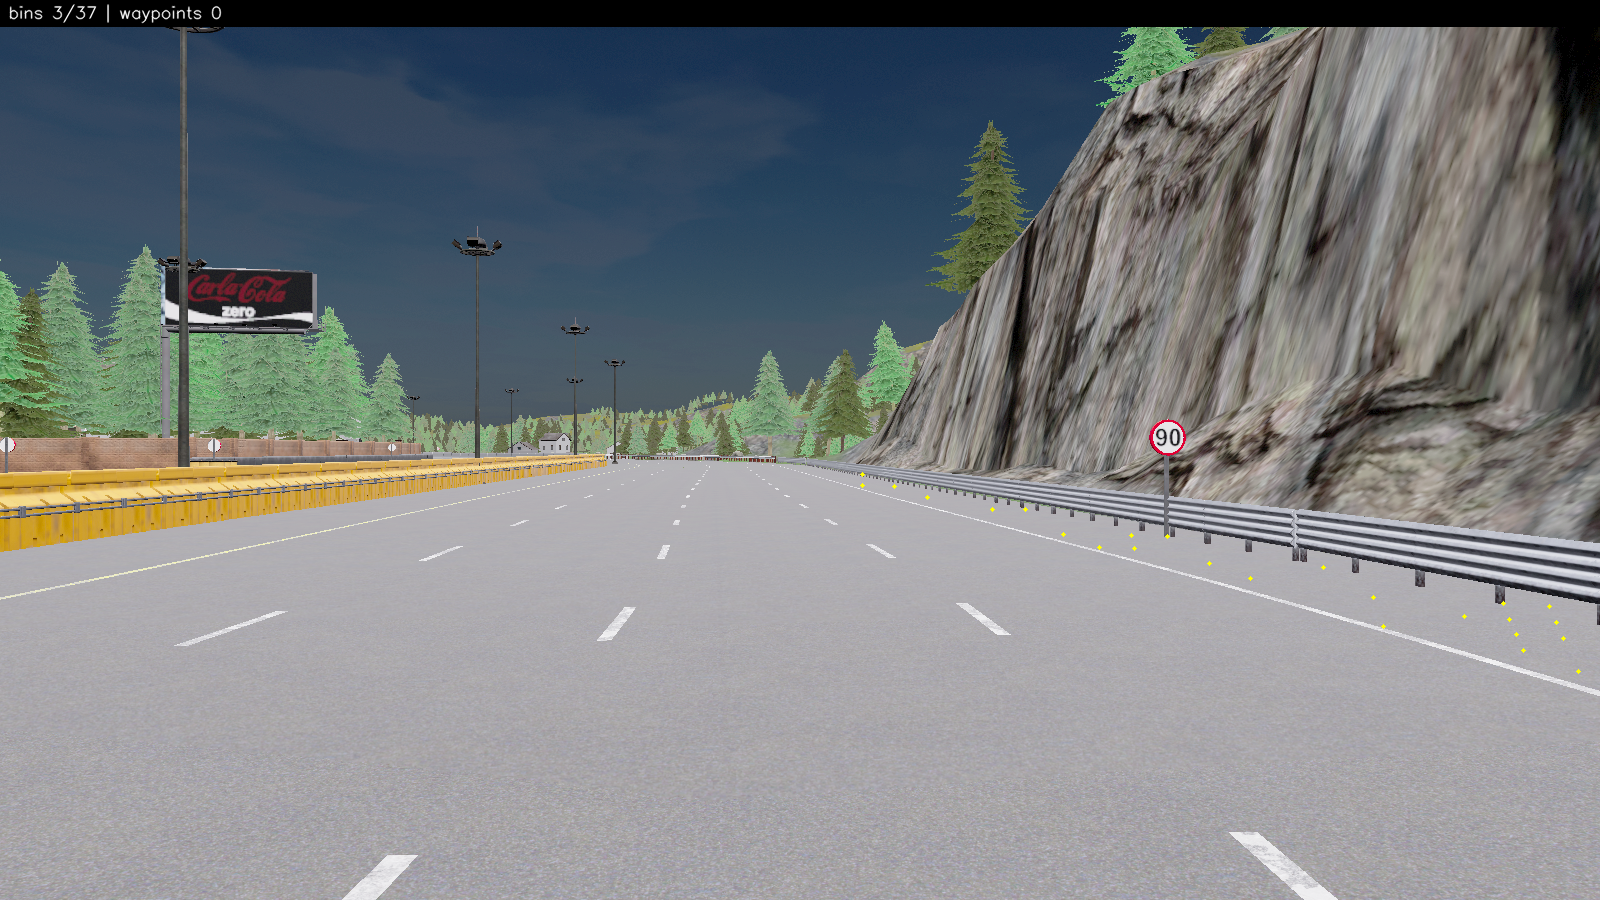
\includegraphics[width=0.75\linewidth]{figs/fig_debug_narrow.png}
\caption{Debug visualization on the same section: yellow dots are LiDAR points landing on the
shoulder-classified mask region (Section~\ref{sec:pointpainting}); the magenta polyline is the
locally fitted centerline reprojected back into the image for sanity-checking, per the project's
established preference for 2D debug views over 3D world-space projection.}
\end{figure}

\begin{figure}[H]
\centering
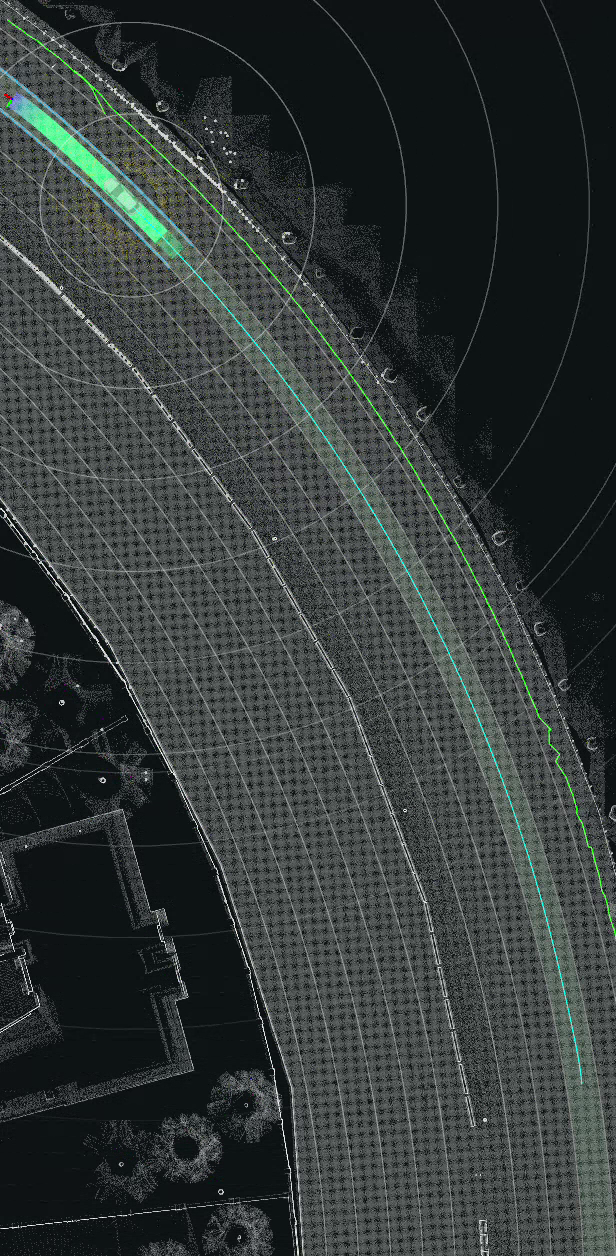
\includegraphics[width=0.6\linewidth]{figs/fig_accumulated_good.png}
\caption{A long, established stretch of the accumulated map-frame path (thin, wavy-free green line)
alongside Autoware's own planned trajectory (cyan), overlaid on the live LiDAR point cloud in RViz.}
\end{figure}

\section{Software Architecture Summary}

The implementation is a standalone \code{ament\_cmake} C++ package, \code{shoulder\_centerline},
deliberately independent of the existing Python/PyTorch inference package for execution speed and
to avoid competing for the same contended GPU. Table~\ref{tab:params} summarizes the introduced
runtime parameters (all launch-time configurable, no rebuild required to change).

\begin{table}[H]
\centering
\small
\begin{tabular}{@{}llp{7.7cm}@{}}
\toprule
\textbf{Parameter} & \textbf{Default} & \textbf{Purpose} \\
\midrule
\code{bin\_source} & \code{mask\_ipm} & Selects Section~\ref{sec:pointpainting} (\code{lidar}) or \ref{sec:ipm} (\code{mask\_ipm}) grounding. \\
\code{centerline\_estimator} & \code{extent\_midpoint} & Selects Eq.~\ref{eq:extentmid} vs.\ plain median per bin. \\
\code{edge\_trim\_fraction} & 0.1 & Trim fraction in Eq.~\ref{eq:extentmid}. \\
\code{x\_min}, \code{x\_max}, \code{bin\_size} & 3.0, 40.0, 1.0\,m & Forward-distance binning window. \\
\code{min\_points\_per\_bin} & 3 & Density gate per local bin. \\
\code{waypoint\_spacing} & 1.0\,m & Arclength spacing of output waypoints. \\
\code{smoothing\_alpha} & 0.3 & EMA factor, local path. \\
\code{accumulate\_path} & true & Enables the world-frame accumulated path. \\
\code{min\_world\_bin\_samples} & 20 & Maturation gate before a world bin publishes. \\
\code{world\_min\_capture\_x} & 10.0\,m & Absolute capture-distance gate, Eq.~\ref{eq:capturegate}. \\
\code{max\_accumulated\_points} & 2000 & Caps retained world bins (oldest dropped first). \\
\bottomrule
\end{tabular}
\caption{Key runtime-configurable parameters introduced in \code{shoulder\_centerline}.}
\label{tab:params}
\end{table}

\subsection{Version Control as a Safety Net}
Because several of the refinements in Section~\ref{sec:refinements} were tried and reverted, the
previously-uncontrolled workspace was placed under \code{git} version control specifically to make
this safe: every non-trivial change was committed as its own checkpoint, and reverting to a known
good state was done as a new revert commit (\code{git checkout \textless commit\textgreater{} --
src/} followed by a commit), preserving the reverted work in history rather than discarding it,
should any part prove worth revisiting.

\section{Conclusion}

Ego-relative shoulder centerline waypoints are generated by 3D-grounding a 2D semantic mask (via
either LiDAR semantic painting or monocular ground-plane IPM), estimating a robust lateral center
per forward-distance bin, fitting a natural cubic spline for the local/real-time path, and
separately accumulating raw grounded samples into a persistent, world-anchored trail keyed by
traveled arclength. The most effective single change for narrow-shoulder robustness was switching
the grounding method from sparse LiDAR painting to dense mask-boundary IPM
(Section~\ref{sec:ipm}); the most effective change for the accumulated path's long-run accuracy was
an absolute (not rank-based) capture-distance trust gate (Eq.~\ref{eq:capturegate}), motivated by
the well-documented near-range error growth of monocular IPM.

\begin{thebibliography}{9}

\bibitem{vora2020pointpainting}
S.~Vora, A.~H.~Lang, B.~Helou, and O.~Beijbom, ``PointPainting: Sequential Fusion for 3D Object
Detection,'' in \emph{Proc.\ IEEE/CVF Conf.\ on Computer Vision and Pattern Recognition (CVPR)},
Seattle, WA, USA, 2020, pp.\ 4604--4612.

\bibitem{ipm2021}
Alternative Inverse Perspective Mapping Homography Matrix Computation for ADAS Systems Using
Camera Intrinsic and Extrinsic Calibration Parameters, \emph{Ain Shams Engineering Journal /
ScienceDirect}, 2021.

\bibitem{ipm2026}
Enhancing Inverse Perspective Mapping for Automatic Vectorized Road Map Generation, \emph{arXiv
preprint arXiv:2601.19536}, 2026.

\bibitem{theil1950}
H.~Theil, ``A Rank-Invariant Method of Linear and Polynomial Regression Analysis,'' \emph{Nederl.\
Akad.\ Wetensch.\ Proc.}, vol.\ 53, pp.\ 386--392, 521--525, 1397--1412, 1950.

\bibitem{sen1968}
P.~K.~Sen, ``Estimates of the Regression Coefficient Based on Kendall's Tau,'' \emph{Journal of
the American Statistical Association}, vol.\ 63, no.\ 324, pp.\ 1379--1389, 1968.

\bibitem{numericalrecipes}
W.~H.~Press, S.~A.~Teukolsky, W.~T.~Vetterling, and B.~P.~Flannery, \emph{Numerical Recipes: The
Art of Scientific Computing}, 3rd ed. Cambridge University Press, 2007, ch.\ 3 (Interpolation and
Extrapolation -- cubic spline interpolation).

\bibitem{autowarepp}
Autoware Foundation, \emph{autoware\_image\_projection\_based\_fusion: pointpainting\_fusion},
Autoware Universe documentation.

\end{thebibliography}

\end{document}
